% Created 2017-01-27 Fri 14:08
% Intended LaTeX compiler: pdflatex
\documentclass[presentation,smaller]{beamer}
\RequirePackage{etex}
\RequirePackage[l2tabu,orthodox]{nag}            %% Warn about obsolete commands and packages
\RequirePackage{amsmath,amsfonts,amssymb,amsthm} %% Math
\RequirePackage{ifxetex,ifluatex}                %% Detect XeTeX and LuaTeX
\RequirePackage{fixltx2e}                        %% provides \textsubscript
\RequirePackage{xspace}
\RequirePackage{graphicx}
\RequirePackage{comment}
\RequirePackage{url}
\RequirePackage{relsize}
\RequirePackage{booktabs}
\RequirePackage{tabularx}
\RequirePackage[normalem]{ulem}
\RequirePackage[all]{xy}
\RequirePackage{etoolbox}

%%%
%%% Code Listings
%%%

\RequirePackage{listings}
\lstdefinelanguage{Sage}[]{Python}{morekeywords={True,False,sage,cdef,cpdef,ctypedef,self},sensitive=true}

\lstset{frame=none,
  showtabs=False,
  showspaces=False,
  showstringspaces=False,
  commentstyle={\color{gray}},
  keywordstyle={\color{mLightBrown}\textbf},
  stringstyle ={\color{mDarkBrown}},
  frame=single,
  basicstyle=\tt\scriptsize\relax,
  backgroundcolor=\color{gray!190!black},
  inputencoding=utf8,
  literate={…}{{\ldots}}1,
  belowskip=0.0em,
}

\makeatletter
\patchcmd{\@verbatim}
  {\verbatim@font}
  {\verbatim@font\scriptsize}
  {}{}
\makeatother

%%%
%%% Tikz
%%%

\RequirePackage{tikz,pgfplots}

\usetikzlibrary{calc}
\usetikzlibrary{arrows}
\usetikzlibrary{automata}
\usetikzlibrary{positioning}
\usetikzlibrary{decorations.pathmorphing}
\usetikzlibrary{backgrounds}
\usetikzlibrary{fit,}
\usetikzlibrary{shapes.symbols}
\usetikzlibrary{chains}
\usetikzlibrary{shapes.geometric}
\usetikzlibrary{shapes.arrows}
\usetikzlibrary{graphs}

%% Cache

\ifdefined\tikzcaching  % chktex 1
  \usetikzlibrary{external}
  \tikzexternalize[prefix=build/]
  \tikzset{external/up to date check=diff}  %% MD5 fails from within emacs
\fi

%%%
%%% SVG (Inkscape)
%%%

\ifxetex % chktex 1
\newcommand{\executeiffilenewer}[3]{%
  {\immediate\write18{#3}} % hack
}
\else
\newcommand{\executeiffilenewer}[3]{%
  \ifnum\pdfstrcmp{\pdffilemoddate{#1}}%
    {\pdffilemoddate{#2}}>0%
    {\immediate\write18{#3}}
  \fi%
}
\fi

\newcommand{\includesvg}[2][1.0\textwidth]{%
 \executeiffilenewer{#1.svg}{#1.pdf}%
 {inkscape -z -D --file=#2.svg --export-pdf=#2.pdf --export-latex --export-area-page}%
 \def\svgwidth{#1} 
 \input{#2.pdf_tex}%
} 

%%%
%%% Metropolis Theme
%%%

\usetheme{metropolis}
\metroset{color/block=fill}
\metroset{numbering=none}
\metroset{outer/progressbar=foot}
\metroset{titleformat=smallcaps}

\setbeamercolor{description item}{fg=mLightBrown}
% \setbeamerfont{alerted text}{series=\bfseries}
\setbeamerfont{footnote}{size=\scriptsize}
\setbeamercolor{example text}{fg=mDarkBrown}

\renewcommand*{\UrlFont}{\ttfamily\smaller\relax}

%%%
%%% UTF-8
%%% 

\RequirePackage{unicodesymbols} % after metropolis which loads fontspec

%%%
%%% BibLaTeX
%%%

\RequirePackage[backend=bibtex,
            style=alphabetic,
            maxnames=4,
            citestyle=alphabetic]{biblatex}

\bibliography{local.bib,abbrev3.bib,crypto_crossref.bib,rfc.bib,jacm.bib}

\DeclareFieldFormat{title}{\alert{#1}}
\DeclareFieldFormat[book]{title}{\alert{#1}}
\DeclareFieldFormat[thesis]{title}{\alert{#1}}
\DeclareFieldFormat[inproceedings]{title}{\alert{#1}}
\DeclareFieldFormat[incollection]{title}{\alert{#1}}
\DeclareFieldFormat[article]{title}{\alert{#1}}
\DeclareFieldFormat[misc]{title}{\alert{#1}}

%%% 
%%% Microtype
%%%

\IfFileExists{upquote.sty}{\RequirePackage{upquote}}{}
\IfFileExists{microtype.sty}{\RequirePackage{microtype}}{}

\setlength{\parindent}{0pt}                   %%
\setlength{\parskip}{6pt plus 2pt minus 1pt}  %%
\setlength{\emergencystretch}{3em}            %% prevent overfull lines
\setcounter{secnumdepth}{0}                   %%

%%% Local Variables:
%%% mode: latex
%%% End:
\usepackage{graphicx}
\usepackage{grffile}
\usepackage{longtable}
\usepackage{wrapfig}
\usepackage{rotating}
\usepackage[normalem]{ulem}
\usepackage{amsmath}
\usepackage{textcomp}
\usepackage{amssymb}
\usepackage{capt-of}
\usepackage{hyperref}
\usepackage{microtype}
\usepackage{newunicodechar}
\usepackage{unicodesymbols}
\usepackage[notions,operators,sets,keys,ff,adversary,primitives,complexity,asymptotics,lambda,landau,advantage]{cryptocode}
\usepackage{xspace}
\usepackage{units}
\usepackage{nicefrac}
\usepackage{gensymb}
\usepackage{amsthm}
\usepackage{amsmath}
\usepackage{amssymb}
\usepackage{xcolor}
\usepackage{listings}
\usepackage[color=yellow!40]{todonotes}
\usepackage{etoolbox}
\makeatletter
\patchcmd{\@verbatim}
{\verbatim@font}
{\verbatim@font\scriptsize}
{}{}
\makeatother
\newcommand{\cR}{\ensuremath{\mathcal{R}}\xspace}
\newcommand{\Z}{\ensuremath{\mathbb Z}\xspace}
\renewcommand{\C}{\ensuremath{\mathbb C}\xspace}
\newcommand{\R}{\ensuremath{\mathbb R}\xspace}
\newcommand{\K}{\ensuremath{\mathbb K}\xspace}
\renewcommand{\L}{\ensuremath{\mathbb L}\xspace}
\newcommand{\Q}{\ensuremath{\mathbb Q}\xspace}
\newcommand{\OK}{\ensuremath{\mathcal O_{\K}}\xspace}
\newcommand{\OL}{\ensuremath{\mathcal O_{\L}}\xspace}
\usetheme{default}
\author{Martin R. Albrecht and Léo Ducas}
\date{Oxford Lattice School}
\title{Sage for Lattice-based Cryptography}
\hypersetup{
pdfauthor={Martin R. Albrecht and Léo Ducas},
pdftitle={Sage for Lattice-based Cryptography},
pdfkeywords={},
pdfsubject={},
pdfcreator={Emacs 25.1.1 (Org mode 9.0.3)},
pdflang={English},
colorlinks,
citecolor=gray,
filecolor=gray,
linkcolor=gray,
urlcolor=gray
}
\begin{document}

\maketitle
\begin{frame}{Outline}
\tableofcontents
\end{frame}



\section{Sage}
\label{sec:org73ad163}
\begin{frame}[label={sec:org55d92a3}]{Blurb}
\begin{columns}
\begin{column}{0.15\columnwidth}
\begin{center}
\begin{center}

\includegraphics[height=0.9\textwidth]{./sage-logo.png}
\end{center}
\end{center}
\end{column}

\begin{column}{0.8\columnwidth}
\begin{block}{Sage open-source mathematical software system}
“Creating a viable free open source alternative to Magma, Maple, Mathematica and Matlab.”
\end{block}
\end{column}
\end{columns}

Sage is a free open-source mathematics software system licensed under the GPL. It combines the power of many existing open-source packages into a common Python-based interface.
\end{frame}

\begin{frame}[fragile,label={sec:orge2b7552}]{How to use it}
 \begin{description}
\item[{command line}] run \texttt{sage}
\item[{local webapp}] run \texttt{sage -notebook=jupyter}
\item[{hosted webapp}] \url{https://cloud.sagemath.com} \footnote{On SMC you have the choice between “Sage Worksheet” and “Jupyter Notebook”. We recommend the latter.}
\item[{widget}] \url{http://sagecell.sagemath.org}
\end{description}
\end{frame}

\begin{frame}[label={sec:orgc2a86f6}]{Python \& Cython}
\begin{center}
\centering
\begin{center}

\includegraphics[width=0.6\textwidth]{./python-and-cython.png}
\end{center}
\end{center}

Sage does \alert{not} come with yet-another ad-hoc mathematical programming language, it uses \alert{Python} instead.

\begin{itemize}
\item one of the most widely used programming languages (Google, IML, NASA, Dropbox),
\item easy for you to define your own data types and methods on it (bitstreams, lattices, cyclotomic rings, …),
\item very clean language that results in easy to read code,
\item a \alert{huge number of libraries}: statistics, networking, databases, bioinformatic, physics, video games, 3d graphics, numerical computation (SciPy), and pure mathematic
\item easy to use existing C/C++ libraries from Python (via \alert{Cython})
\end{itemize}
\end{frame}

\begin{frame}[fragile,label={sec:org855ec46}]{Sage ≠ Python}
 \begin{columns}[t]
\begin{column}{0.45\columnwidth}
\textbf{Sage}

\lstset{language=sage,label= ,caption= ,captionpos=b,numbers=none}
\begin{lstlisting}
1/2
\end{lstlisting}

\begin{verbatim}
1/2
\end{verbatim}

\lstset{language=sage,label= ,caption= ,captionpos=b,numbers=none}
\begin{lstlisting}
2^3
\end{lstlisting}

\begin{verbatim}
8
\end{verbatim}

\lstset{language=sage,label= ,caption= ,captionpos=b,numbers=none}
\begin{lstlisting}
type(2)
\end{lstlisting}

\begin{verbatim}
<type 'sage.rings.integer.Integer'>
\end{verbatim}
\end{column}

\begin{column}{0.45\columnwidth}
\textbf{Python}

\lstset{language=Python,label= ,caption= ,captionpos=b,numbers=none}
\begin{lstlisting}
1/2
\end{lstlisting}

\begin{verbatim}
0
\end{verbatim}

\lstset{language=Python,label= ,caption= ,captionpos=b,numbers=none}
\begin{lstlisting}
2^3
\end{lstlisting}

\begin{verbatim}
1
\end{verbatim}

\lstset{language=Python,label= ,caption= ,captionpos=b,numbers=none}
\begin{lstlisting}
type(2)
\end{lstlisting}

\begin{verbatim}
<type 'int'>
\end{verbatim}
\end{column}
\end{columns}
\end{frame}

\begin{frame}[fragile,label={sec:orgdb3fa6b}]{Sage ≠ Python}
 \begin{columns}[t]
\begin{column}{0.45\columnwidth}
\textbf{Sage}

\lstset{language=sage,label= ,caption= ,captionpos=b,numbers=none}
\begin{lstlisting}
type(2r)
\end{lstlisting}

\begin{verbatim}
<type 'int'>
\end{verbatim}

\lstset{language=sage,label= ,caption= ,captionpos=b,numbers=none}
\begin{lstlisting}
type(range(10)[0])
\end{lstlisting}

\begin{verbatim}
<type 'int'>
\end{verbatim}
\end{column}

\begin{column}{0.45\columnwidth}
\textbf{Python}

\lstset{language=Python,label= ,caption= ,captionpos=b,numbers=none}
\begin{lstlisting}
type(2r)
\end{lstlisting}

\begin{verbatim}
SyntaxError: invalid syntax
\end{verbatim}

\lstset{language=Python,label= ,caption= ,captionpos=b,numbers=none}
\begin{lstlisting}
type(range(10)[0])
\end{lstlisting}

\begin{verbatim}
<type 'int'>
\end{verbatim}
\end{column}
\end{columns}


\begin{block}{Files}
\texttt{.sage} files are parsed as Sage code, \texttt{.py} files as Python code
\end{block}
\end{frame}


\begin{frame}[fragile,allowframebreaks]{Naive RSA}
 \lstset{language=sage,label= ,caption= ,captionpos=b,numbers=none}
\begin{lstlisting}
sage: p, q = random_prime(2^512), random_prime(2^512)
sage: n = p*q
sage: ZZn = IntegerModRing(n)
\end{lstlisting}

\lstset{language=sage,label= ,caption= ,captionpos=b,numbers=none}
\begin{lstlisting}
sage: r = (p-1)*(q-1)
sage: ZZr = IntegerModRing(r)
\end{lstlisting}

\lstset{language=sage,label= ,caption= ,captionpos=b,numbers=none}
\begin{lstlisting}
sage: e = ZZ.random_element(r)
sage: while gcd(e, r) != 1:
         e = ZZ.random_element(r)
\end{lstlisting}

\framebreak{}

\lstset{language=sage,label= ,caption= ,captionpos=b,numbers=none}
\begin{lstlisting}
sage: type(e)
\end{lstlisting}

\begin{verbatim}
<type 'sage.rings.integer.Integer'>
\end{verbatim}

\lstset{language=sage,label= ,caption= ,captionpos=b,numbers=none}
\begin{lstlisting}
sage: type(ZZr(e))
\end{lstlisting}

\begin{verbatim}
<type 'sage.rings.finite_rings.integer_mod.IntegerMod_gmp'>
\end{verbatim}

\lstset{language=sage,label= ,caption= ,captionpos=b,numbers=none}
\begin{lstlisting}
sage: d = ZZr(e)^-1
sage: m = ZZn.random_element()
sage: s = m^e
sage: s^d == m
\end{lstlisting}

\begin{verbatim}
True
\end{verbatim}
\end{frame}

\begin{frame}[fragile,allowframebreaks]{Sage has Algebraic Types}
 Objects know the field, ring, group etc. where they live. We say that \textbf{elements} know their \textbf{parents}:

\lstset{language=sage,label= ,caption= ,captionpos=b,numbers=none}
\begin{lstlisting}
sage: parent(2)
\end{lstlisting}

\begin{verbatim}
Integer Ring
\end{verbatim}

\lstset{language=sage,label= ,caption= ,captionpos=b,numbers=none}
\begin{lstlisting}
sage: K = GF(3)
sage: e = K(2)
sage: parent(e)
\end{lstlisting}

\begin{verbatim}
Finite Field of size 3
\end{verbatim}

\framebreak

Elements follow the rules of their parents:

\lstset{language=sage,label= ,caption= ,captionpos=b,numbers=none}
\begin{lstlisting}
sage: 2 + 3
\end{lstlisting}

\begin{verbatim}
5
\end{verbatim}

\lstset{language=sage,label= ,caption= ,captionpos=b,numbers=none}
\begin{lstlisting}
sage: e, f = K(2), K(3)
sage: e + f
\end{lstlisting}

\begin{verbatim}
2
\end{verbatim}

\framebreak

If there is a canonical map between parents, it is applied implicitly

\lstset{language=sage,label= ,caption= ,captionpos=b,numbers=none}
\begin{lstlisting}
sage: e + 3
\end{lstlisting}

\begin{verbatim}
2
\end{verbatim}

\lstset{language=sage,label= ,caption= ,captionpos=b,numbers=none}
\begin{lstlisting}
sage: v = random_vector(ZZ['x'], 2)
sage: w = random_vector(GF(7), 2)
sage: v + w
\end{lstlisting}

\begin{verbatim}
(2*x^2 + 6, 4*x + 5)
\end{verbatim}

\framebreak

Otherwise, an error is raised:

\lstset{language=sage,label= ,caption= ,captionpos=b,numbers=none}
\begin{lstlisting}
sage: L = GF(5)
sage: K(2) + L(3)
\end{lstlisting}

\begin{verbatim}
TypeError: unsupported operand parent(s) for '+': 
'Finite Field of size 3' and 'Finite Field of size 5'
\end{verbatim}

See \url{http://doc.sagemath.org/html/en/tutorial/tour\_coercion.html} for details

\framebreak

Somewhat annoyingly for lattice-based cryptography, Sage likes to normalise to \([0,\ldots,q-1]\) instead of \([\lceil -q/2 \rceil,\ldots, \lfloor q/2 \rfloor]\)

\lstset{language=sage,label= ,caption= ,captionpos=b,numbers=none}
\begin{lstlisting}
sage: K = GF(101)
sage: K(-1)
\end{lstlisting}

\begin{verbatim}
100
\end{verbatim}

\lstset{language=sage,label= ,caption= ,captionpos=b,numbers=none}
\begin{lstlisting}
sage: ZZ(K(-1))
\end{lstlisting}

\begin{verbatim}
100
\end{verbatim}

\framebreak

\lstset{language=sage,label= ,caption= ,captionpos=b,numbers=none}
\begin{lstlisting}
def balance(e, q=None):
    try:
        p = parent(e).change_ring(ZZ)
        return p([balance(e_) for e_ in e])
    except (TypeError, AttributeError):
        if q is None:
            try:
                q = parent(e).order()
            except AttributeError:
                q = parent(e).base_ring().order()
        return ZZ(e)-q if ZZ(e)>q/2 else ZZ(e)

balance(GF(101)(60))
balance(random_vector(GF(101), 2))
balance(PolynomialRing(GF(101), 'x').random_element(degree=3))
\end{lstlisting}

\begin{itemize}
\item \(-41\)
\item \(\left(-47,\,31\right)\)
\item \(34x^{3} - 20x^{2} + 11x - 48\)
\end{itemize}
\end{frame}

\begin{frame}[fragile,allowframebreaks]{Symbolic Manipulation}
 Sage also supports symbolic manipulation

\begin{itemize}
\item We define some symbols and make assumptions about them:

\lstset{language=sage,label= ,caption= ,captionpos=b,numbers=none}
\begin{lstlisting}
n, alpha, q, epsilon, delta_0 = var("n, alpha, q, epsilon, delta_0")
assume(alpha<1)
\end{lstlisting}

\item We compute the expected norm of the shortest vector found via lattice reduction with \(δ_0\)

\lstset{language=sage,label= ,caption= ,captionpos=b,numbers=none}
\begin{lstlisting}
e = alpha*q/sqrt(2*pi) # stddev
m = 2*n # lattice dimension
v = e * delta_0^m * q^(n/m)  # norm of the vector
\end{lstlisting}

\framebreak

\item Use advantage \footfullcite{RSA:LinPei11} \(ε = \exp\left(-π⋅(\|v\|/q)^2\right)\) and solve for \(\log δ_0\):

\lstset{language=sage,label= ,caption= ,captionpos=b,numbers=none}
\begin{lstlisting}
f = log(1/epsilon)/pi == (v/q)^2
f = f.solve(delta_0**(2*m))[0]
f = f.log().canonicalize_radical()
f = f.solve(log(delta_0))[0]
f.simplify_log()
\end{lstlisting}
\end{itemize}

\begin{center}
\(\log\left(\delta_{0}\right) = \frac{\log\left(-\frac{2 \, \log\left(\epsilon\right)}{\alpha^{2} q}\right)}{4 \, n}\)
\end{center}
\end{frame}

\begin{frame}[fragile,label={sec:org6c6a6be}]{Dense Linear Algebra}
 \lstset{language=sage,label= ,caption= ,captionpos=b,numbers=none}
\begin{lstlisting}
sage: for p in (2,3,4,7,8,9,11):
         K = GF(p, 'a')
         n = 2000 if p != 9 else 500
         A, B = (random_matrix(K, n, n) for _ in range(2))
         t = cputime()
         C = A*B
         print "%32s %10.8f"%(K,cputime(t))
\end{lstlisting}

\begin{center}
\begin{tabular}{lrl}
Field & Time & Implementation\\
\hline
Finite Field of size 2 & 0.004 s & \href{https://bitbucket.org/malb/m4rie}{M4RI}\\
Finite Field of size 3 & 0.212 s & \href{http://www.linalg.org}{LinBox}\\
Finite Field in a of size \(2^2\) & 0.020 s & \href{https://bitbucket.org/malb/m4rie}{M4RIE}\\
Finite Field of size 7 & 0.208 s & \href{http://www.linalg.org}{LinBox}\\
Finite Field in a of size \(2^3\) & 0.040 s & \href{https://bitbucket.org/malb/m4rie}{M4RIE}\\
Finite Field in a of size \(3^2\) & \alert{7.28 s} & generic\\
Finite Field of size 11 & 0.212 s & \href{http://www.linalg.org}{LinBox}\\
\end{tabular}

\end{center}
\end{frame}

\section{Lattices}
\label{sec:org9b6d47f}
\begin{frame}[fragile,label={sec:org0ba46b9}]{Integer Matrices}
 The usual operations on matrices are available:

\lstset{language=sage,label= ,caption= ,captionpos=b,numbers=none}
\begin{lstlisting}
sage: A = random_matrix(ZZ, 100, 100, x=-2^32, y=2^32)
sage: A*A
\end{lstlisting}

\begin{verbatim}
100 x 100 dense matrix over Integer Ring \
  (use the '.str()' method to see the entries)
\end{verbatim}

\lstset{language=sage,label= ,caption= ,captionpos=b,numbers=none}
\begin{lstlisting}
sage: A = random_matrix(ZZ, 100, 100, x=-2^32, y=2^32)
sage: A.norm().log(2).n()
\end{lstlisting}

\begin{verbatim}
35.4775417878382
\end{verbatim}

\lstset{language=sage,label= ,caption= ,captionpos=b,numbers=none}
\begin{lstlisting}
sage: abs(A.det()).log(2).n()
\end{lstlisting}

\begin{verbatim}
3380.14491067801
\end{verbatim}
\end{frame}

\begin{frame}[fragile,label={sec:org12a9dda}]{Bases for q-ary Lattices}
 We construct a basis for a \(q\)-lattice.

\begin{itemize}
\item We pick parameters

\lstset{language=sage,label= ,caption= ,captionpos=b,numbers=none}
\begin{lstlisting}
m, n, q = 5, 3, 101
\end{lstlisting}

\item We compute the reduced row-echelon form of \(A\)

\lstset{language=sage,label= ,caption= ,captionpos=b,numbers=none}
\begin{lstlisting}
A = random_matrix(GF(q), n, m)
A.echelonize()
\end{lstlisting}

\item We stack \(A\) on top of a matrix accounting for modular reductions

\lstset{language=sage,label= ,caption= ,captionpos=b,numbers=none}
\begin{lstlisting}
N = A.change_ring(ZZ)
S = matrix(ZZ, m-n, n).augment(q * identity_matrix(m-n))
N.stack(S, subdivide=True)
\end{lstlisting}

\small
\(\left(\begin{array}{rrrrr}
  1 & 0 & 0 & 3 & 68 \\
  0 & 1 & 0 & 4 & 96 \\
  0 & 0 & 1 & 30 & 16 \\
  \hline
   0 & 0 & 0 & 101 & 0 \\
  0 & 0 & 0 & 0 & 101
  \end{array}\right)\)
\end{itemize}
\end{frame}

\begin{frame}[fragile,label={sec:orgee02f79}]{Instance Generator}
 If you just want some typical lattices to play with:

\lstset{language=sage,label= ,caption= ,captionpos=b,numbers=none}
\begin{lstlisting}
sage: sage.crypto.gen_lattice(m=10, seed=42, type="modular")
\end{lstlisting}

\begin{verbatim}
[11  0  0  0  0  0  0  0  0  0]
[ 0 11  0  0  0  0  0  0  0  0]
[ 0  0 11  0  0  0  0  0  0  0]
[ 0  0  0 11  0  0  0  0  0  0]
[ 2  4  3  5  1  0  0  0  0  0]
[ 1 -5 -4  2  0  1  0  0  0  0]
[-4  3 -1  1  0  0  1  0  0  0]
[-2 -3 -4 -1  0  0  0  1  0  0]
[-5 -5  3  3  0  0  0  0  1  0]
[-4 -3  2 -5  0  0  0  0  0  1]
\end{verbatim}
\end{frame}

\begin{frame}[fragile,label={sec:org3a97b29}]{LLL}
 LLL is available. By default Sage calls \texttt{Fplll}, but you can also call \texttt{NTL}.

\lstset{language=sage,label= ,caption= ,captionpos=b,numbers=none}
\begin{lstlisting}
sage: A = sage.crypto.gen_lattice(m=10, seed=42, type="modular")
sage: A.LLL(delta=0.99, eta=0.51) # calls fplll
\end{lstlisting}

\begin{verbatim}
[ 0  0  1  1  0 -1 -1 -1  1  0]
[-1  1  0  1  0  1  1  0  1  1]
[-1  0  0  0 -1  1  1 -2  0  0]
[-1 -1  0  1  1  0  0  1  1 -1]
[ 1  0 -1  0  0  0 -2 -2  0  0]
[ 2 -1  0  0  1  0  1  0  0 -1]
[-1  1 -1  0  1 -1  1  0 -1 -2]
[ 0  0 -1  3  0  0  0 -1 -1 -1]
[ 0 -1  0 -1  2  0 -1  0  0  2]
[ 0  1  1  0  1  1 -2  1 -1 -2]
\end{verbatim}

If you want LLL on Gram matrices, \texttt{Pari} is also available.
\end{frame}

\begin{frame}[fragile,label={sec:org84627a9}]{BKZ}
 BKZ is available. By default \texttt{Fplll} is called, but you can also call \texttt{NTL}

\lstset{language=sage,label= ,caption= ,captionpos=b,numbers=none}
\begin{lstlisting}
sage: A = sage.crypto.gen_lattice(m=100, seed=42, q=next_prime(2^20))
sage: B = A.BKZ(block_size=60, proof=False) # calls fplll's BKZ 2.0
sage: B[0].norm().log(2).n()
\end{lstlisting}

\begin{verbatim}
2.26178097802851
\end{verbatim}

\begin{block}{Note}
Passing \texttt{proof=False} enables BKZ 2.0 with some decent heuristics. It will be much faster than \texttt{proof=True} which reverts back to plain BKZ without any pruning or recursive preprocessing.
\end{block}
\end{frame}

\begin{frame}[fragile,label={sec:orgf9b3230}]{Lattices}
 Sometimes it is more natural to work with a lattice object directly, instead of a basis matrix\footnote{Lattices are still represented by bases, though.}

\lstset{language=sage,label= ,caption= ,captionpos=b,numbers=none}
\begin{lstlisting}
sage: from sage.modules.free_module_integer import IntegerLattice
sage: A = random_matrix(ZZ, 80, 80, x=-2000, y=2000)
sage: L = IntegerLattice(A); L
\end{lstlisting}

\begin{verbatim}
Free module of degree 80 and rank 80 over Integer Ring
User basis matrix:
80 x 80 dense matrix over Integer Ring
\end{verbatim}

\lstset{language=sage,label= ,caption= ,captionpos=b,numbers=none}
\begin{lstlisting}
sage: L.shortest_vector().norm().log(2).n()
\end{lstlisting}

\begin{verbatim}
13.1049884393931
\end{verbatim}
\end{frame}

\begin{frame}[fragile,label={sec:org32213a5}]{Discrete Gaussians: Integers}
 Discrete Gaussian samplers are available as:

\lstset{language=sage,label= ,caption= ,captionpos=b,numbers=none}
\begin{lstlisting}
sage: from sage.stats.distributions.discrete_gaussian_integer import \
  DiscreteGaussianDistributionIntegerSampler
sage: D = DiscreteGaussianDistributionIntegerSampler(3.2)
sage: histogram([D() for _ in range(2^16)], color="orange")
\end{lstlisting}

\begin{center}
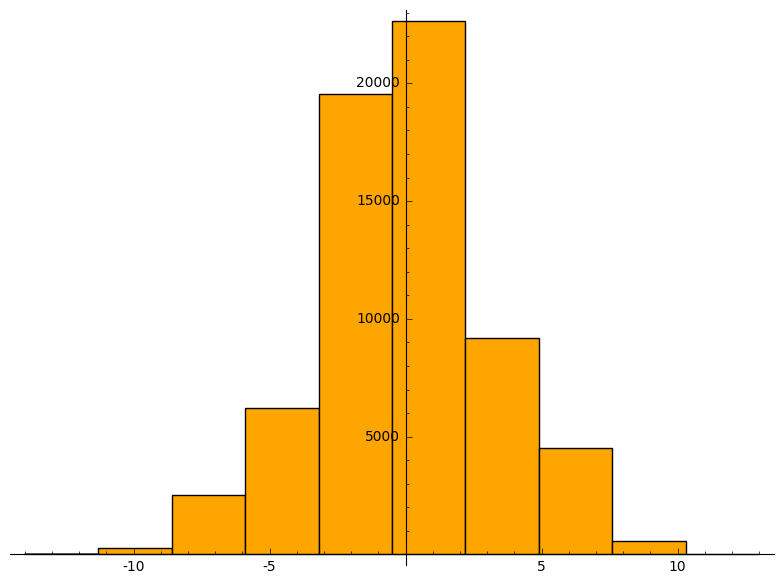
\includegraphics[width=0.5\textwidth]{discrete-gaussian-integer.png}
\end{center}
\end{frame}

\begin{frame}[fragile,label={sec:orgcfba929}]{Discrete Gaussians: Lattices}
 GPV algorithm for sampling from arbitrary lattices.\footfullcite{STOC:GenPeiVai08}

\lstset{language=sage,label= ,caption= ,captionpos=b,numbers=none}
\begin{lstlisting}
sage: from sage.stats.distributions.discrete_gaussian_lattice import \
   DiscreteGaussianDistributionLatticeSampler
sage: A = random_matrix(ZZ, 2, 2)
sage: D = DiscreteGaussianDistributionLatticeSampler(A, 20.0)
sage: S = [D() for _ in range(2^12)]
sage: l = [vector(v.list() + [S.count(v)]) for v in set(S)]
sage: list_plot3d(l, point_list=True, interpolation='nn')
\end{lstlisting}

\begin{center}
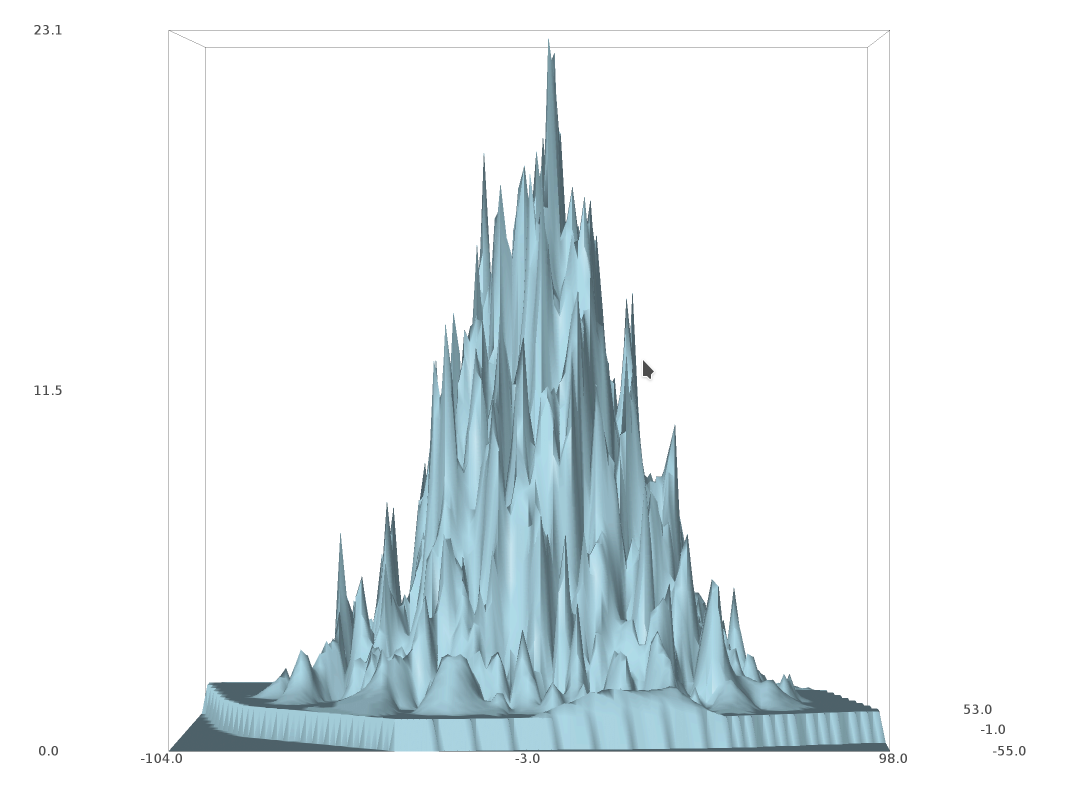
\includegraphics[width=0.4\textwidth]{./discrete-gaussian-lattice.png}
\end{center}
\end{frame}

\begin{frame}[fragile,label={sec:orgbdab677}]{Learning with Errors}
 \begin{itemize}
\item Module also has \texttt{Regev} and \texttt{LindnerPeikert} samplers

\lstset{language=sage,label= ,caption= ,captionpos=b,numbers=none}
\begin{lstlisting}
sage: from sage.crypto.lwe import LWE
\end{lstlisting}

\item We need a noise distribution sampler

\lstset{language=sage,label= ,caption= ,captionpos=b,numbers=none}
\begin{lstlisting}
sage: D = DiscreteGaussianDistributionIntegerSampler(3.2) # stddev
\end{lstlisting}

\item We can optionally also pass in the number \(m\) of supported samples

\lstset{language=sage,label= ,caption= ,captionpos=b,numbers=none}
\begin{lstlisting}
sage: lwe = LWE(n=10, q=101, D=D)
\end{lstlisting}

\item Get a sample and decrypt

\lstset{language=sage,label= ,caption= ,captionpos=b,numbers=none}
\begin{lstlisting}
sage: a,c = lwe()
sage: balance(c - a*lwe._LWE__s)
\end{lstlisting}

\begin{verbatim}
-4
\end{verbatim}
\end{itemize}
\end{frame}

\begin{frame}[fragile,allowframebreaks]{fpylll}
 \texttt{Fpylll} is a Python frontend for \texttt{Fplll}, giving access to its internals. It’s main aim is to facilitate experiments with lattice reduction.

\lstset{language=sage,label= ,caption= ,captionpos=b,numbers=none}
\begin{lstlisting}
sage: from fpylll import *
sage: A = IntegerMatrix(50, 50)
sage: A.randomize("ntrulike", bits=50, q=127)
sage: A[0].norm()
\end{lstlisting}

\begin{verbatim}
394.37418779631105
\end{verbatim}

\framebreak

\begin{itemize}
\item We create a Gram-Schmidt object for orthogonalisation

\lstset{language=sage,label= ,caption= ,captionpos=b,numbers=none}
\begin{lstlisting}
sage: M = GSO.Mat(A)
sage: _ = M.update_gso()
sage: M.get_mu(1,0)
\end{lstlisting}

\begin{verbatim}
0.7982010017295588
\end{verbatim}

\item We create an LLL object that actos on \texttt{M}

\lstset{language=sage,label= ,caption= ,captionpos=b,numbers=none}
\begin{lstlisting}
sage: L = LLL.Reduction(M)
sage: L()
sage: M.get_mu(1,0)
\end{lstlisting}

\begin{verbatim}
0.24
\end{verbatim}

\item Operations on \texttt{M} are also applied to \texttt{A}

\lstset{language=sage,label= ,caption= ,captionpos=b,numbers=none}
\begin{lstlisting}
sage: A[0].norm()
\end{lstlisting}

\begin{verbatim}
5.0
\end{verbatim}
\end{itemize}
\end{frame}

\begin{frame}[fragile,allowframebreaks]{fpylll: BKZ}
 \lstset{language=sage,label= ,caption= ,captionpos=b,numbers=none}
\begin{lstlisting}
class BKZReduction:
    def __init__(self, A):
        self.A = A
        self.m = GSO.Mat(A, flags=GSO.ROW_EXPO)
        self.lll_obj = LLL.Reduction(self.m)
\end{lstlisting}

\lstset{language=sage,label= ,caption= ,captionpos=b,numbers=none}
\begin{lstlisting}
    def __call__(self, block_size):
        self.m.discover_all_rows()

        while True:
            clean = self.bkz_loop(block_size, 0, self.A.nrows)
            if clean:
                break
\end{lstlisting}

\lstset{language=sage,label= ,caption= ,captionpos=b,numbers=none}
\begin{lstlisting}
    def bkz_loop(self, block_size, min_row, max_row):
        clean = True
        for kappa in range(min_row, max_row-1):
            bs = min(block_size, max_row - kappa)
            clean &= self.svp_reduction(kappa, bs)
        return clean
\end{lstlisting}

\framebreak

\lstset{language=sage,label= ,caption= ,captionpos=b,numbers=none}
\begin{lstlisting}
    def svp_reduction(self, kappa, block_size):
        clean = True

        self.lll_obj(0, kappa, kappa + block_size)
        if self.lll_obj.nswaps > 0:
            clean = False

        max_dist, expo = self.m.get_r_exp(kappa, kappa)
        delta_max_dist = self.lll_obj.delta * max_dist

        solution, max_dist = Enumeration(self.m).enumerate(kappa, \
                               kappa + block_size, \
                               max_dist, expo, pruning=None)[0]
\end{lstlisting}

\framebreak

\lstset{language=sage,label= ,caption= ,captionpos=b,numbers=none}
\begin{lstlisting}
        if max_dist >= delta_max_dist * (1<<expo):
            return clean

        nonzero_vectors = len([x for x in solution if x])

        if nonzero_vectors == 1:
            first_nonzero_vector = None
            for i in range(block_size):
                if abs(solution[i]) == 1:
                    first_nonzero_vector = i
                    break

            self.m.move_row(kappa + first_nonzero_vector, kappa)
            self.lll_obj.size_reduction(kappa, \
                  kappa + first_nonzero_vector + 1)
\end{lstlisting}

\framebreak

\lstset{language=sage,label= ,caption= ,captionpos=b,numbers=none}
\begin{lstlisting}
        else:
            d = self.m.d
            self.m.create_row()

            with self.m.row_ops(d, d+1):
                for i in range(block_size):
                    self.m.row_addmul(d, kappa + i, solution[i])

            self.m.move_row(d, kappa)
            self.lll_obj(kappa, kappa, kappa + block_size + 1)
            self.m.move_row(kappa + block_size, d)

            self.m.remove_last_row()

        return False
\end{lstlisting}
\end{frame}


\section{Rings}
\label{sec:org45e5daa}
\begin{frame}[fragile,allowframebreaks]{Polynomial Rings}
 \begin{itemize}
\item Sage has polynomial rings …

\lstset{language=sage,label= ,caption= ,captionpos=b,numbers=none}
\begin{lstlisting}
sage: P = ZZ['x']; x = P.gen()
sage: P = PolynomialRing(ZZ, 'x'); x = P.gen()
sage: P, x = PolynomialRing(ZZ, 'x').objgen()
sage: P.<x> = PolynomialRing(ZZ) # not valid Python, Magma-style
\end{lstlisting}

\item … over arbitrary rings

\lstset{language=sage,label= ,caption= ,captionpos=b,numbers=none}
\begin{lstlisting}
sage: R = PolynomialRing(P, 'y'); R
sage: R = PolynomialRing(IntegerModRing(100), 'y'); R
sage: R = PolynomialRing(GF(2^8,'a'), 'x'); R
\end{lstlisting}

\begin{verbatim}
Univariate Polynomial Ring in y over \
  Univariate Polynomial Ring in x over Integer Ring
Univariate Polynomial Ring in y over Ring of integers modulo 100
Univariate Polynomial Ring in x over Finite Field in a of size 2^8
\end{verbatim}
\end{itemize}

\framebreak

\begin{itemize}
\item It also supports multivariate polynomial rings

\lstset{language=sage,label= ,caption= ,captionpos=b,numbers=none}
\begin{lstlisting}
sage: R = PolynomialRing(QQ, 'x,y'); R
sage: R.<x,y> = PolynomialRing(QQ); R
sage: R = PolynomialRing(QQ, 2, 'x'); R
sage: names = ["x%02d"%i for i in range(3)]
sage: R = PolynomialRing(IntegerModRing(100), names); R
\end{lstlisting}

\begin{verbatim}
Multivariate Polynomial Ring in x, y over Rational Field
Multivariate Polynomial Ring in x, y over Rational Field
Multivariate Polynomial Ring in x0, x1 over Rational Field
Multivariate Polynomial Ring in x00, x01, x02 \
 over Ring of integers modulo 100
\end{verbatim}
\end{itemize}
\end{frame}
\begin{frame}[fragile,label={sec:orgfc869fa}]{Quotient Rings}
 \begin{itemize}
\item You can construct quotient rings:

\lstset{language=sage,label= ,caption= ,captionpos=b,numbers=none}
\begin{lstlisting}
sage: P.<x> = PolynomialRing(ZZ)
sage: Q = P.quotient(x^4 + 1); Q
\end{lstlisting}

\begin{verbatim}
Univariate Quotient Polynomial Ring in xbar \
  over Integer Ring with modulus x^4 + 1
\end{verbatim}

\item But I usually don’t bother and do modular reductions “by hand”:

\lstset{language=sage,label= ,caption= ,captionpos=b,numbers=none}
\begin{lstlisting}
sage: P.<x> = PolynomialRing(ZZ)
sage: f = P.random_element(degree=5); f
sage: f % (x^4 + 1)
\end{lstlisting}

\begin{verbatim}
x^5 + 9*x^4 + x^3 + x^2 + 2
x^3 + x^2 - x - 7
\end{verbatim}
\end{itemize}
\end{frame}

\begin{frame}[fragile,label={sec:org9431624}]{Number Fields}
 \begin{itemize}
\item Relative and absolute number fields are a thing:

\lstset{language=sage,label= ,caption= ,captionpos=b,numbers=none}
\begin{lstlisting}
sage: z = QQ['z'].0
sage: K = NumberField(z^2 - 2,'s'); K
\end{lstlisting}

\begin{verbatim}
Number Field in s with defining polynomial z^2 - 2
\end{verbatim}

\lstset{language=sage,label= ,caption= ,captionpos=b,numbers=none}
\begin{lstlisting}
sage: s = K.0; s
\end{lstlisting}

\begin{verbatim}
s
\end{verbatim}

\lstset{language=sage,label= ,caption= ,captionpos=b,numbers=none}
\begin{lstlisting}
sage: s^2
\end{lstlisting}

\begin{verbatim}
2
\end{verbatim}
\end{itemize}
\end{frame}

\begin{frame}[fragile,label={sec:orge6a8fd1}]{Cyclotomic Number Fields}
 Let \(\cR ≃ \Z[X]/(X^{n}+1)\) be the ring of integers of the Cylotomic number field \(\K = \Q(ζ_m)\) for some \(m=2^k\) and \(n = m/2\).

\lstset{language=sage,label= ,caption= ,captionpos=b,numbers=none}
\begin{lstlisting}
sage: K.<zeta> = CyclotomicField(8)
sage: OK = K.ring_of_integers()
sage: K.polynomial()
\end{lstlisting}

\begin{verbatim}
x^4 + 1
\end{verbatim}
\end{frame}

\begin{frame}[fragile,label={sec:orgb0e9819}]{Cyclotomic Number Fields: Subfields}
 Let \(\L = \Q(ζ_{m'})\) with \(m' | m\) be a subfield of \(\K\). The ring of integers of \(\L\) is \(\cR' ≃ \Z[X]/(X^{n'} + 1)\) with \(n' = m'/2\).

\lstset{language=sage,label= ,caption= ,captionpos=b,numbers=none}
\begin{lstlisting}
sage: KK, L = K.subfield(zeta^2)
sage: zeta_ = KK.gen()
sage: L(zeta_)
\end{lstlisting}

\begin{verbatim}
zeta^2
\end{verbatim}
\end{frame}

\begin{frame}[fragile,label={sec:org6376d91}]{Cyclotomic Number Fields: Galois Group}
 \(\K\) is a Galois extension of \(\Q\), and its Galois group \(G\) is isomorphic to \(\Z_m^*\): \(i \in \Z_m^* \leftrightarrow (X \mapsto X^i) \in G\).

\lstset{language=sage,label= ,caption= ,captionpos=b,numbers=none}
\begin{lstlisting}
sage: G = K.galois_group(); G
\end{lstlisting}

\begin{verbatim}
Galois group of Cyclotomic Field of order 8 and degree 4
\end{verbatim}
\end{frame}

\begin{frame}[fragile,label={sec:org108575d}]{Cyclotomic Number Fields: Class Group}
 The first Cyclotomic field with \(m=2^k\) and a non-trivial class group is \(m=2^6\).

\lstset{language=sage,label= ,caption= ,captionpos=b,numbers=none}
\begin{lstlisting}
sage: K.<zeta> = CyclotomicField(2^6)
sage: K.class_number(proof=False)
\end{lstlisting}

\begin{verbatim}
17
\end{verbatim}
\end{frame}

\begin{frame}[fragile,label={sec:orgf561498}]{Cyclotomic Number Fields: Lattices}
 \begin{itemize}
\item Converting number field elements to matrices/lattice bases:

\lstset{language=sage,label= ,caption= ,captionpos=b,numbers=none}
\begin{lstlisting}
sage: from sage.modules.free_module_integer import IntegerLattice
sage: f
sage: IntegerLattice(f).basis_matrix()
\end{lstlisting}

\begin{verbatim}
-10*zeta^3 + 2*zeta + 28

[ 28   2   0 -10]
[ 10  28   2   0]
[  0  10  28   2]
[ -2   0  10  28]
\end{verbatim}

\item We can use this to find small elements

\lstset{language=sage,label= ,caption= ,captionpos=b,numbers=none}
\begin{lstlisting}
sage: K = CyclotomicField(128)
sage: OK = K.ring_of_integers()
sage: f = OK.random_element(x=-128, y=128)
sage: L = IntegerLattice(f)
sage: _ = L.BKZ(block_size=50, proof=False)
sage: L.shortest_vector().norm().log(2).n()
\end{lstlisting}

\begin{verbatim}
9.23365749434346
\end{verbatim}
\end{itemize}
\end{frame}

\begin{frame}[standout,label={sec:org6d919a8}]{Fin}
\begin{center}
{\Huge \alert{Thank You} }
\end{center}
\end{frame}
\end{document}